% !TEX root = ../../main.tex

\subsection{Thermal stability}

In order to check if the shaped samples have not undergone bulk
structural changes, as well as find a suitable activation temperature,
the powder and shaped samples underwent thermogravimetric analysis
under an argon atmosphere.

\begin{figure}
	\centering
	\begin{subfigure}{0.85\textwidth}
		\parbox[c]{0.1\linewidth}{\caption{}\label{shaping:fig:tgauio66}}%
		\parbox[b]{0.7\linewidth}{%
			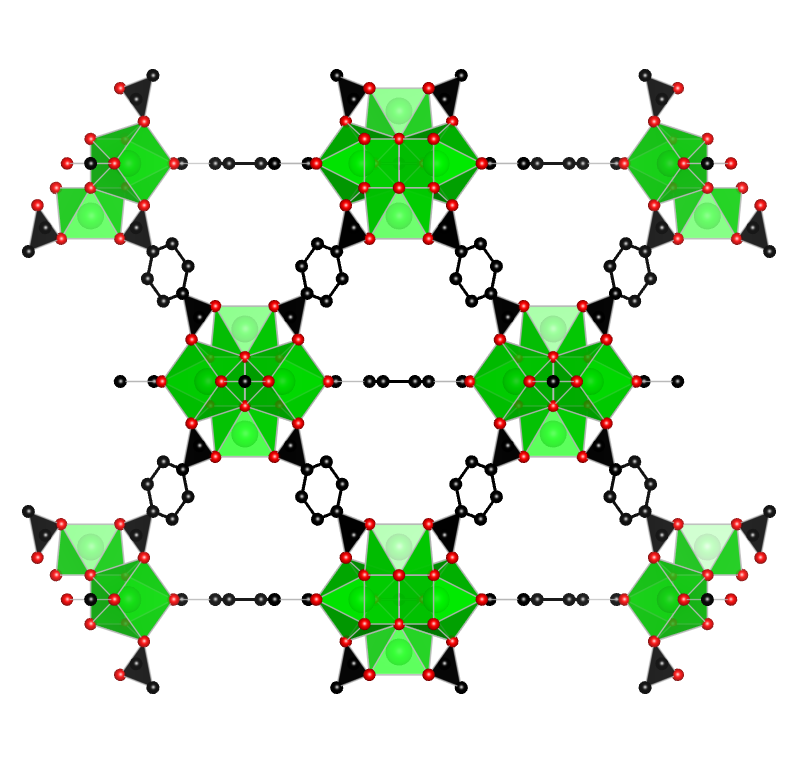
\includegraphics[width=\linewidth]{tga/uio66}%
		}%
	\end{subfigure}%

	\begin{subfigure}{0.85\textwidth}
		\parbox[c]{0.1\linewidth}{\caption{}\label{shaping:fig:tgamil100}}%
		\parbox[b]{0.7\linewidth}{%
			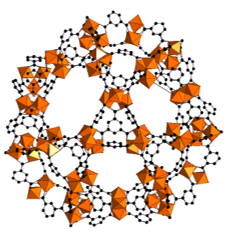
\includegraphics[width=\linewidth]{tga/mil100}%
		}%
	\end{subfigure}%
	
	\begin{subfigure}{0.85\textwidth}
		\parbox[c]{0.1\linewidth}{\caption{}\label{shaping:fig:tgamil127}}%
		\parbox[b]{0.7\linewidth}{%
			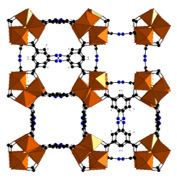
\includegraphics[width=\linewidth]{tga/mil127}%
		}%
	\end{subfigure}%

	\caption{High resolution TGA curves recoded under argon
		on (a) UiO-66(Zr), (b) MIL-100(Fe) and (c) MIL-127(Fe). The
		original powders are depicted in red and the shaped material
		in blue.}%
	\label{shaping:fig:tgacurves}

\end{figure}

The process of shaping did not have any impact on the thermal stability of
the investigated MOFs, as evidenced by the TGA curves in
\autoref{shaping:fig:tgacurves}. The primary mass loss occurs
in a \SI{10}{\kelvin} range for all powder-pellet pairs.
Shaped samples are also seen to have a smaller mass loss
at high temperatures. This is expected, as after the addition of
temperature inert alumina, the MOF makes up a lower percentage of
the material.